\documentclass[11pt, oneside]{article}
\usepackage[letterpaper, margin=2cm]{geometry}
\usepackage{MATH520}

\begin{document}
\noindent \textbf{\Large{Caleb Logemann \\
MATH 520 Methods of Applied Math II \\
Homework 9
}}

\subsection*{Section 14.5}
\begin{enumerate}
  \item[\#5]
    Let $Lu = a_2(x) u'' + a_1(x)u' + a_0(x) u$ with $a_2' = a$, so that $L$ is
    formally self adjoint.
    If $B_1 u = C_1 u(a) + C_2u'(a)$, $B_2 u = C_3u(b) + C_4u'(b)$, show that
    $\set{B_1^*, B_2^*} = \set{B_1, B_2}$.

    \begin{proof}
      Let $\set{B_1^*, B_2^*}$ be the set of boundary operators adjoint to
      $\set{B_1, B_2}$.
      This implies that
      \[
        \eval{J(\phi, \psi)}{a}{b} = 0
      \]
      whenever $B_1 \phi = B_2 \phi = B_1^* \psi = B_2^* \psi = 0$.
      The boundary function $J$ can be expressed as
      \[
        J(\phi, \psi) = a_2\p{\phi' \overline{\psi} - \phi \overline{\psi'}} + (a_1 - a_2') \phi \overline{\psi}
      \]
      and since $L$ is formally self-adjoint, this implies that $a_1 - a_2' = 0$,
      so the boundary functional can be simplified to
      \[
        J(\phi, \psi) = a_2\p{\phi' \overline{\psi} - \phi \overline{\psi'}}.
      \]
    \end{proof}

  \pagebreak
  \item[\#8]
    When we rewrite $a_2(x) u'' + a_1(x) u' + a_0(x) u = \lambda u$ as
    \[
      -(p(x)u')' + q(x)u = \lambda \rho(x) u
    \]
    the latter is often referred to as the \textit{Liouville normal form}.
    Consider the eigenvalue problem
    \[
      x^2 u'' + xu' + u = \lambda u \qquad 1 < x < 2
    \]
    \[
      u(1) = u(2) = 0
    \]
    \begin{enumerate}
      \item[(a)] % Done
        Find the Liouville normal form.

        In order to find the Liouville normal form, the function $a_2(x)$ must
        be strictly less than zero, so I will first rewrite this eigenvalue
        problem as
        \[
          -x^2 u'' - xu' - u = -\lambda u \qquad 1 < x < 2
        \]
        \[
          u(1) = u(2) = 0
        \]
        The functions $p(x)$, $\rho(x)$, and $q(x)$ can be found as follows.
        \begin{align*}
          p(x) &= \exp\p{\dintt{a}{x}{\frac{a_1(s)}{a_2(s)}}{s}} \\
          &= \exp\p{\dintt{a}{x}{\frac{-s}{-s^2}}{s}} \\
          &= \exp\p{\dintt{a}{x}{\frac{1}{s}}{s}} \\
          &= \exp\p{\eval{\ln{s}}{s = a}{x}} \\
          &= e^{\ln{x} - \ln{a}} \\
          &= e^{\ln{\frac{x}{a}}} \\
          &= \frac{x}{a} \\
          \rho(x) &= - \frac{p(x)}{a_2(x)} \\
          &= - \frac{x/a}{-x^2} \\
          &= \frac{1}{ax} \\
          q(x) &= a_0(x) \rho(x) \\
          &= (-1)\frac{1}{ax}\\
          &= -\frac{1}{ax}\\
        \end{align*}
        Therefore the Liouville normal form of this eigenvalue problem is
        \[
          -\p{\frac{x}{a} \phi'}' - \frac{1}{ax} \phi = -\lambda \frac{1}{ax} \phi
        \]
        or 
        \[
          \p{\frac{x}{a} \phi'}' + \frac{1}{ax} \phi = \lambda \frac{1}{ax} \phi
        \]

      \item[(b)] % Done
        What is the orthogonality relationship satisfied by the eigenfunctions?

        The eigenfunctions of this linear operator satisfy an orthogonality
        relationship with respect to the weight $\rho$.
        In mathematical terms,
        \[
          \dintt{a}{b}{\phi_n(x) \phi_m(x) \rho(x)}{x} =
          \begin{cases}
            0 & n \neq m \\
            1 & n = m
          \end{cases}
        \]
        or
        \[
          \dintt{a}{b}{\frac{\phi_n(x) \phi_m(x)}{ax}}{x} =
          \begin{cases}
            0 & n \neq m \\
            1 & n = m
          \end{cases}
        \]

      \item[(c)]
        Find the eigenvalues and eigenfunctions.
        (You may find the original form of the equation easier to work with than
        the Liouville normal form when computing the eigenvalues and
        eigenfunctions.)

        
    \end{enumerate}

  \pagebreak
  \item[\#10]
    Consider the Sturm-Liouville problem
    \begin{align*}
      u'' + \lambda u = 0 \qquad 0 < x < 1 \\
      u(0) - u'(0) = u(1) = 0
    \end{align*}
    \begin{enumerate}
      \item[(a)] % Done
        Multiply the equation by $u$ and integrate by parts to show that any
        eigenvalue is positive.

        First I will note a few useful facts, first since $u(0) - u'(0) = 0$,
        this implies that $u(0) = u'(0)$.
        Also if $u$ is nontrivial this guarantees that
        $\dintt{0}{1}{u^2(x)}{x} > 0$.
        Finally if $u$ is a nontrivial solution then $u'(x) \neq 0$ as
        $u(1) = 0$ makes any constant function is zero.
        This shows that $\dintt{0}{1}{\p{u'(x)}^2}{x} > 0$ as well.

        Multiplying by $u$ gives the following equation
        \[
          uu'' + \lambda u^2 = 0.
        \]
        Integrating both sides over $\br{0, 1}$ gives
        \[
          \dintt{0}{1}{u(x)u''(x)}{x} + \lambda \dintt{0}{1}{u^2(x)}{x} = \dintt{0}{1}{0}{x}
        \]
        This can be simplified using integration by parts
        \begin{align*}
          \dintt{0}{1}{u(x)u''(x)}{x} + \lambda \dintt{0}{1}{u^2(x)}{x} &= 0 \\
          \eval{u(x)u'(x)}{x = 0}{1} - \dintt{0}{1}{\p{u'(x)}^2}{x} + \lambda \dintt{0}{1}{u^2(x)}{x} &= 0 \\
          u(1)u'(1) - u(0)u'(0) - \dintt{0}{1}{\p{u'(x)}^2}{x} + \lambda \dintt{0}{1}{u^2(x)}{x} &= 0
          \intertext{Since $u(1) = 0$ and $u(0) = u'(0)$}
           -u^2(0) - \dintt{0}{1}{\p{u'(x)}^2}{x} + \lambda \dintt{0}{1}{u^2(x)}{x} &= 0.
        \end{align*}
        Since $\dintt{0}{1}{u^2(x)}{x} > 0$
        \[
          \lambda = \frac{u^2(0) + \dintt{0}{1}{\p{u'(x)}^2}{x}}{\dintt{0}{1}{u^2(x)}{x}} > 0.
        \]

      \item[(b)]
        Show that the eigenvalues are the positive solutions of
        $\tan{\sqrt{\lambda}} = - \sqrt{\lambda}$.

      \item[(c)]
        Show graphically that such roots exist, and form an infinite sequence
        $\lambda_k$ such that $(k - 1/2)\pi < \sqrt{\lambda_k} < k \pi$ and
        \[
          \lim[k \to \infty]{\sqrt{\lambda_k} - (k - 1/2)\pi} = 0
        \]

        First this graph shows that solutions to the equation
        $\tan{\sqrt{\lambda}} = -\sqrt{\lambda}$ exist.
        \begin{center}
          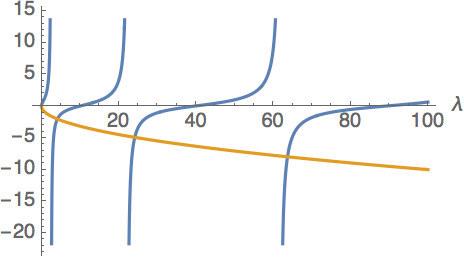
\includegraphics[scale=.5]{Figures/09_1}
        \end{center}

        Next
    \end{enumerate}

  \pagebreak
  \item[\#14]
    If $\set{\psi_n}_{n = 1}^{\infty}$ are Dirichlet eigenfunctions of the
    Laplacian making up an orthonormal basis of $L^2(\Omega)$, let
    $\xi_n = \psi_n/\sqrt{\lambda_n}$
    ($\lambda_n$ the corresponding eigenvalue).
    \begin{enumerate}
      \item[(a)]
        Show that $\set{\xi_n}_{n = 1}^{\infty}$ is an orthonormal basis of
        $H^1_0(\Omega)$.

      \item[(b)]
        Show that $f \in H_0^1(\Omega)$ if and only if
        $\sum{n = 1}{\infty}{\lambda_n \abs{\abr{f, \psi_n}}^2} < \infty$
    \end{enumerate}

  \pagebreak
  \item[\#15]
    If $\Omega < \RR^n$ is a bounded open set with smooth enough boundary, find
    a solution of the wave equation problem
    \begin{align*}
      u_{tt} - \Delta u = 0 \qquad x \in \Omega \quad t > 0 \\
      u(x, t) = 0 \qquad x \in \partial\Omega \quad t > 0 \\
      u(x, 0) = f(x) \quad u_t(x, 0) = g(x) \qquad x \in \Omega
    \end{align*}
    in the form
    \[
      u(x, t) = \sum{n = 1}{\infty}{c_n(t) \psi_n(x)}
    \]
    where $\set{\psi_n}_{n = 1}^{\infty}$ are the Dirichlet eigenfunctions of
    $-\Delta$ in $\Omega$.

  \pagebreak
  \item[\#16]
    Derive formally that
    \[
      G(x, y) = \sum{n=1}{\infty}{\frac{\psi_n(x) \psi_n(y)}{\lambda_n}}
    \]
    where $\lambda_n, \psi_n$ are the Dirichlet eigenvalues and normalized
    eigenfunctions for the domain $\Omega$, and $G(x, y)$ is the corresponding
    Green's function in (14.4.96).
    (Suggestion: if $-\Delta u = f$, expand both $u$ and $f$ in the $\psi_n$
    basis.)
\end{enumerate}
\end{document}
